\documentclass[12pt, a4paper]{article}

\usepackage[utf8]{inputenc}

% Limit the page margin to only 1 inch.
\usepackage[margin=1in]{geometry}

%Imports biblatex package
\usepackage[
backend=biber,
style=alphabetic
]{biblatex}
\addbibresource{../math-342w.bib}

% Enables the `align' environment.
\usepackage{amsmath}
\allowdisplaybreaks
\usepackage{bm}
\usepackage{array}
\usepackage{rotating}
\usepackage{multirow}

% Provides useful environments, such as:
% - \begin{proof} ...\end{proof}
\usepackage{amsthm}
\newtheorem{proposition}{Proposition}
\theoremstyle{definition}
\newtheorem*{definition}{Definition}
\newtheorem{theorem}{Theorem}
\newtheorem{corollary}{Corollary}
\newtheorem*{example}{Example}
\newtheorem{algorithm}{Algorithm}

% Enables using \mathbb{}, for example \mathbb{N} for the set of natural numbers.
\usepackage{amssymb}

% Allows using letters in enumerate list environment. Use, for example:
%\begin{enumerate}[label=(\alph*)]
% ...
%\end{enumerate}
\usepackage[inline]{enumitem}

% Enable importing external graphic files and provides useful commands, like \graphicspath{}
\usepackage{graphicx}
% Images are located in a directory called "images" in the current directory.
\graphicspath{{./images/}}

% Make links look better by default.
% See: https://tex.stackexchange.com/questions/823/remove-ugly-borders-around-clickable-cross-references-and-hyperlinks
\usepackage[hidelinks]{hyperref}
\usepackage{xcolor}
\hypersetup{
	colorlinks,
	linkcolor={red!50!black},
	citecolor={blue!50!black},
	urlcolor={blue!80!black}
}

% Code Listings. Source:
% https://stackoverflow.com/questions/3175105/inserting-code-in-this-latex-document-with-indentation
\usepackage{listings}
\usepackage{color}
\usepackage[most]{tcolorbox}

\definecolor{dkgreen}{rgb}{0,0.6,0}
\definecolor{gray}{rgb}{0.5,0.5,0.5}
\definecolor{mauve}{rgb}{0.58,0,0.82}

\lstset{frame=tb,
	language=Java,
	aboveskip=3mm,
	belowskip=3mm,
	showstringspaces=false,
	columns=flexible,
	basicstyle={\small\ttfamily},
	numbers=none,
	numberstyle=\tiny\color{gray},
	keywordstyle=\color{blue},
	commentstyle=\color{dkgreen},
	stringstyle=\color{mauve},
	breaklines=true,
	breakatwhitespace=true,
	tabsize=3
}

\title{Lecture 22: MATH 342W: Introduction to Data Science and Machine Learning}
\author{Sergio E. Garcia Tapia\thanks{Based on lectures of Dr. Adam Kapelner at Queens College.
See also the \href{https://github.com/kapelner/QC_MATH_342W_Spring_2025}{course GitHub page}.}}
\date{May 1st, 2025 (last updated \today)}

\begin{document}
	\maketitle
	\section{Missingness}
	Last time, we began discussing missingness. Recall this means there is
	missingness in $X$, not in $y$'s. If $y$'s are missing, then the unit would
	not be in $\mathbb{D}$. None of the algorithms that we have seen can handle
	missing data.
	
	\subsection{Listwise Deletion}
	The most naive (simple) approach for handling missingness is \textbf{listwise deletion},
	which involves dropping all rows that have missingness. This may be alright if
	a ``trivial" amount of data is missing. However, this there is ``a lot" of missingness,
	listwise deletion can introduce errors in our predictive model.
	
	The first type of error is estimation error because there is less data,
	which an also make us more likely to overfit. But that is not all; if
	there is a pattern to the missing data, then the predictive model is
	prone to poor extrapolation, likely due ot \textbf{sampling bias}.
	For example, one of our features may be age, and it could be that the
	units that are missing correspond to senior-aged individuals
	(see Figure~\ref{fig:model-after-listwise-deletion}).
	\begin{figure}
		\centering
		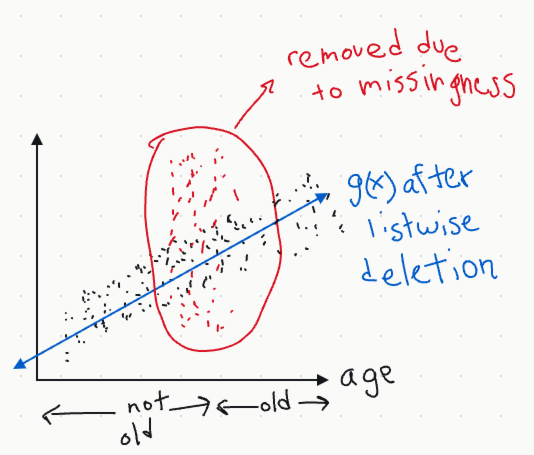
\includegraphics[width=0.4\textwidth]{model-after-listwise-deletion}
		\caption{Computing predictive function $g$ on $\mathbb{D}$ after
		performing listwise deletion.}
		\label{fig:model-after-listwise-deletion}
	\end{figure}
	To know what we should do next, we need to discuss what is known as
	\textbf{missing data mechanisms}.
	\subsection{Missing Data Mechanisms (MDMs)}
	Missing data mechanisms are devised in accordance to the question ``why is $x_{ij}$
	missing?". We will discuss the following possibilities:
	\begin{enumerate}[label=(\arabic*)]
		\item Data is missing completely at random (MCAR).
		\item Data is missing at random (MAR).
		\item Data is not missing at random (NMAR).
	\end{enumerate}
	\subsubsection{Missing Completely At Random (MCAR)}
	Let $M_{ij}$ be the Bernoulli random variable which equals $1$ if $x_{ij}$
	is missing, meaning
	\begin{align*}
		P(M_{ij} = 1 \mid \gamma)
	\end{align*}
	where $\gamma$ is independent of all $X$ and $\bm{y}$ (that is,
	$M \sim \text{Bernoulli}(\gamma)$).
	
	\begin{tcolorbox}[breakable]
		\begin{example}
			MCAR may be the result of data corruption (think of a solid
			state drive subjected to magnetism). This is rare in practice due to
			modernized data storage solutions. Nevertheless, we need a way to deal with
			the possibility.
		\end{example}
	\end{tcolorbox}
	
	The solution is to \textbf{impute} all $x_{ij}$ that are missing. Let
	$\mathcal{M}$ be the set of feature indices that contain missingness
	in some unit. We \textit{predict} values the missing $x_{ij}$ by viewing
	$\bm{x}_{\cdot, j}$, the $j$th column (which has all $n$ values for the $j$th feature)
	as the response; we use $\bm{x}_{\cdot, -j}$ (all other features besides the
	$j$th feature) and $\bm{y}$ as the inputs. This yields an \textbf{imputed design matrix}
	\begin{align*}
		X_{\text{imp}} = \text{Imputed}(X, \bm{y})
	\end{align*}
	Then we apply our methodology as usual to compute a prediction function:
	\begin{align*}
		g = \mathcal{A}(\langle X_{\text{imp}}, \bm{y} \rangle, \mathcal{H})
	\end{align*}
	Why does this work? We are assuming that there is a functional relationship
	between $X$ and $\bm{y}$, which suggests that there is probably some
	way to recover $X$ from $\bm{y}$.
	\subsubsection{Missing At Random (MAR)}
	This means that the probability that $x_{ij}$ is missing is dependent
	not only on $\gamma$ (as in MCAR), but also on all other values for
	the measurements on unit $i$ besides $j$ that are available, as well as values
	of the measurements on unit $i$ that are missing:
	\begin{align*}
		P\left(M_{ij} \mid \gamma, \bm{x}_{i, -j}, \bm{x}_{i, -j_{\text{missing}}}\right)
	\end{align*}
	For example, suppose $i = 3$, $p_{\text{raw}} = 6$, and that a certain unit is
	\begin{align*}
		\bm{x}_i = \begin{bmatrix}
			17.1 & 15.6 & \texttt{NA} & \text{``Blue"} & \texttt{NA} & 7
		\end{bmatrix}
	\end{align*}
	That is, the missingness of one of the features influences the missingness
	of another. In MAR, we also impute.
	
	\begin{tcolorbox}[breakable]
		\begin{example}
			Suppose there is a survey, and a person does not answer a question.
			Perhaps they do not answer because the question does not apply to them, or
			they choose not to for personal reasons, or maybe the person is old and struggles
			to read a question or notice it is there to begin with.
		\end{example}
	\end{tcolorbox}
	\subsubsection{Not Missing At Random (NMAR)}
	In this case, the probability that data is missing is given by
	\begin{align*}
		P\left(
		M_{ij} \mid \gamma, \bm{x}_{\cdot, -j}, \bm{x}_{\cdot, -j_{\text{missing}}},x_{ij}, \vec{U}
		\right)
	\end{align*}
	This is the most general mechanism. Notice the probability depends on $x_{ij}$ too,
	the missing value itself. Here, $\vec{U}$ are the features that are unknown.
	\begin{tcolorbox}[breakable]
		\begin{example}
			Suppose you are the $i$th candidate filling out a survey, and on the
			$j$th question asks whether you spent time in jail, which you decide
			not to answer.
		\end{example}
	\end{tcolorbox}
	In this case, the data is unimputable, but we impute anyway. When imputing,
	it is recommended to create binary variables indicating missingness for all
	indices $\mathcal{M}$.
	
	\begin{tcolorbox}
		\begin{example}
			Suppose $\mathcal{M} = \{3, 7, 11\}$, meaning features indexed $3$, $7$,
			and $11$ have missingness in some units. Then the matrix $M$ might look like
			\begin{align*}
				M = \begin{bmatrix}
					0 & 1 & 1\\
					0 & 0 & 1\\
					0 & 1 & 1\\
					\vdots & \vdots & \vdots\\
					1 & 1 & 0
				\end{bmatrix}
			\end{align*}
			where the first column corresponds to the 3rd feature, the
			second to the 7th feature, and the third to th 11th feature.
		\end{example}
	\end{tcolorbox}
	Entry $M_{ij}$ is $1$ if $x_{ij}$ is missing, and is zero otherwise,
	We treat the columns of $M$ as features and augment matrix $X$
	to $[X \mid M]$. Then we impute on that:
	\begin{align*}
		[X_{\text{imp}} \mid M] = \text{Impute}([X\mid M], \bm{y})
	\end{align*}
	Finally, we compute our predictive model using this augmented matrix:
	\begin{align*}
		g = \mathcal{A}(\langle [X_{\text{mp}}, M], \bm{y}\rangle, \mathcal{H})
	\end{align*}
	The idea is that knowing a feature is missing may carry more information
	than the value of the feature itself had it been present.
	\begin{tcolorbox}
		\begin{example}
			 For example,
			if we are collecting data regarding public school shootings in Chicago
			and a student's GPA is missing, that may be more telling than the
			fact that their GPA is low.
		\end{example}
	\end{tcolorbox}
	In the real world, assume that you should use NMAR.
	\subsection{Imputing}
	How do we actually impute? An imputation really means a prediction,
	but the latter carries the implication that we are predicting on $y$.
	Ultimately, we impute so that we can predict $y$. If $\bm{x}_{\cdot, j}$
	is continuous, binary, or multinomial, then we can use any algorithm
	suitable for continuous, binary, or multinomial responses, respectively.
	Note that random forests can be used for all feature
	types\footnote{Not exactly true, due to survivor features and counts, as you can find
		out by taking MATH 343. However, we will assume it always works here.
	}
	and it is highly accurate.
	
	We can apply the following algorithm to perform imputation.
	\begin{tcolorbox}
		\begin{algorithm}[Miss Forest (2012) Imputation Algorithm]
			Let $\mathcal{M}$ be the set of feature indices for which a
			value is missing in some unit. Let $M$ be the binary matrix
			whose entries indicate missingness for the features encoded by
			$\mathcal{M}$.
			\begin{enumerate}[label=\textbf{(\arabic*)}]
				\setcounter{enumi}{-1}
				\item Initialize the missing values for $\bm{x}_{\cdot, j}$.
				\begin{itemize}
					\item If $\bm{x}_{\cdot, j}$ is continuous, use
					$\text{Average}[\bm{x}_{\cdot, j}]$;
					\item If $\bm{x}_{\cdot, j}$ is categorical, use
					$\text{Mode}[\bm{x}_{\cdot, j}]$.
				\end{itemize}
				\item For all $j\in \mathcal{M}$:
				\begin{itemize}
					\item Let $I_j$ be the row indices for which feature $j$
					does not have missingness. Then let $\bm{x}_{I_j, j}$ be
					the vector of entries of $\bm{x}_{\cdot, j}$ for which no
					values of the $j$th feature are missing.
					Fit
					\begin{align*}
						\bm{x}_{I_j, j}\sim [X_{I_j,-j}\mid M_{I_j, \cdot} \mid \bm{y}_{I_j, \cdot}]
					\end{align*}
					using random forests. That is, treat $\bm{x}_{I_j, j}$ as
					a response, and created an augmented matrix by concatenating
					the columns of $X_{I_j,-j}$, $M_{I_j, \cdot}$, and $\bm{y}_{I_j, \cdot}$
					(The notation above is similar to the R notation for
					$\mathtt{lm(y \sim  X)}$).
					\item Repeat for all features.
					\item Predict $x_{ij}$ for missing values.
				\end{itemize}
				\item Repeat step 1 until 
				\begin{align*}
					\|\bm{x}_t - \bm{x}_{t-1}\| > \|\bm{x}_{t-1} - \bm{x}_{t-2}\|
				\end{align*}
				(that is, continue with imputaton until it cannot do better)
				or $T = 10$ iterations (a default). Let $\bm{x}_t$ be a vector of
				all imputed at iteration $t$.
			\end{enumerate}
		\end{algorithm}
	\end{tcolorbox}
	What if you want a test set? We need a test set to compute honest metrics so that
	we can gauge performance. The reason we have honest metrics is that you have a
	$\bm{y}_{\text{test}}$, which we can compare it to $\hat{\bm{y}}_{\text{test}}$,
	which is like predicting the future.
	
	Suppose we shuffle our data set and cut off a part of it to use as
	$X_{\text{train}}$ and $\bm{y}_{\text{train}}$, and another to use as
	$X_{\text{test}}$ and $\bm{y}_{\text{test}}$:
	\begin{align*}
		&\begin{bmatrix}
			{} & * & {}\\
			{} & X_{\text{train}} & {}\\
			* & {} & {}
		\end{bmatrix}
		\begin{bmatrix}
			{}\\
			\bm{y}_{\text{train}}\\
			{}
		\end{bmatrix}\\
		&\begin{bmatrix}
			* & {} & {}\\
			{} & X_{\text{test}} & {}\\
			{} & * & {}
		\end{bmatrix}
	\end{align*}
	However, if there is missingness
	in $X_{\text{test}}$, what do we do? One thought could be to impute on
	both, but this can get us into trouble because the imputation process involves
	looking at $\bm{y}_{\text{test}}$ to use as a feature. While we can open
	$X_{\text{test}}$, we cannot open $\bm{y}_{\text{test}}$, since it has the
	values that we are trying to predict (see Figure~\ref{fig:train-test-split-missing}).
	\begin{figure}
		\centering
		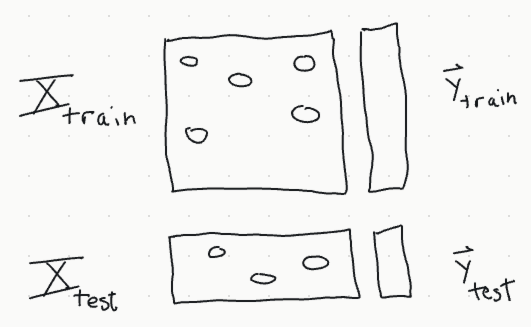
\includegraphics[width=0.4\textwidth]{train-test-split-missingness}
		\caption{The usual split of $\mathbb{D}$ into train and test sets,
		but now we must consider missingness.}
		\label{fig:train-test-split-missing}
	\end{figure}
	To get around this, after splitting, use the whole $X$ (that is $X_{\text{train}}$ and
	$X_{\text{test}}$), and create a $\bm{y}'$ where we keep $\bm{y}_{\text{train}}$
	unchanged by make the $\bm{y}_{\text{test}}$ indices all missing
	(see Figure~\ref{fig:treat-ytest-missing-then-impute}).
	\begin{figure}
		\centering
		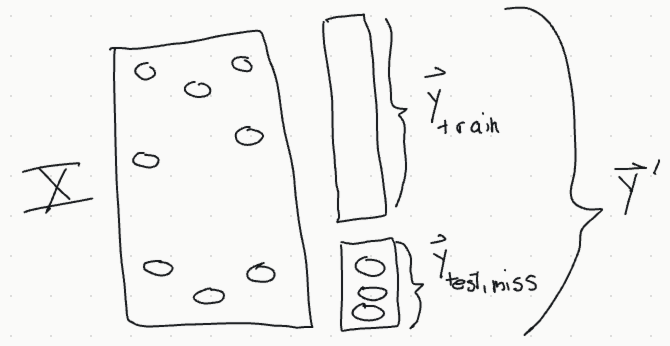
\includegraphics[width=0.5\textwidth]{treating-ytest-as-missing-then-imputing}
		\caption{$X$ concatenates the rows of $X_{\text{train}}$ and $X_{\text{test}}$,
		and $\bm{y}'$ concatenates $\bm{y}_{\text{train}}$ with a vector of missing values
		whose length is that of $\bm{y}_{\text{test}}$.}
		\label{fig:treat-ytest-missing-then-impute}
	\end{figure}
	Then, we will impute on this:
	\begin{align*}
		X_{\text{imp}} = \text{MissForest}(X, \bm{y}')
	\end{align*}
	Note that we do not care what it imputes to for the indices of $\bm{y}_{\text{test}}$;
	we just want to use it to fill in the missing entries in $X$ without relying on the
	actual values of $\bm{y}_{\text{test}}$. Indeed, we need to impute both $X_{\text{train}}$
	and $X_{\text{test}}$, but we do it in such a way that the imputation cannot
	see the future.
	
	This concludes our discussion for missingness, allowing us to apply our algorithms.
	\section{R Demo}
	See \verb|QC_MATH_342W_Spring_2025/practice_lectures/lec22.Rmd|
	(\href{https://github.com/kapelner/QC_MATH_342W_Spring_2025/blob/main/practice_lectures/lec22.Rmd}{click here}).
	\section{Asymmetric Cost Modeling for Binary Classification}
	In our earlier lectures when we introduced binary classification, we did not
	make a distinction between the kind of misclassifications that could occur:
	\begin{align*}
		&\hat{y} = 0,\text{ but } y = 1\quad (\textbf{False Negative (FN)})\\
		&\hat{y} = 1,\text{ but } y = 0\quad (\textbf{False Positive (FP)})
	\end{align*}
	That is, we initially only cared about counting errors, as in our originally
	definition of misclassification error:
	\begin{align*}
		\text{Misclassification Error} := \sum_{i=1}^{n}\mathbb{I}_{y_i \neq \hat{y}_i}
	\end{align*}
	Suppose we denote $C_{FP}$ to mean the cost of a false positive, and $C_{FN}$
	to be the cost of a false negative. In the setting above, $C_{FN}=C_{FP}$, so
	that misclassification error is a suitable function to minimize, but this
	may not always be the case.
	\begin{tcolorbox}
		\begin{example}
			There are many examples of when $C_{FP}\neq C_{FN}$. Among them:
			\begin{itemize}
				\item Consider the binary classification problem of whether a person
				pays back a loan, with a response of $1$ meaning that they will
				pay back. A false positive means we predict they will pay it back,
				so we give them the loan, but instead they up default on the loan. A
				false negative means we predicted they would not pay, but in fact they
				would have paid it back, so we deny them the loan. In this case,
				the false positive is much more costly, so we might have
				$C_{FP} > C_{FN}$.
				\item Suppose we create an authorization system that predicts
				1 if a person is authorized to access a secured facility and 0
				otherwise. A false positive means we say that they are allowed
				to enter but in fact they are not cleared personnel. A false
				negative means we say they are not allowed when in fact they
				have received clearance. The latter is inconvenient but not
				a huge problem; the former might lead to secrets revealed to
				outsiders. In this case, a false positive is again worse than
				a false negative, so $C_{FP} > C_{FN}$.
				\item Consider a fire alarm that goes off, but there is no fire
				(false positive), versus when there is a fire, but the fire
				alarm does not go off (false negative). Here, the false negative
				is most costly, since lives are at stake, so $C_{FN} > C_{FP}$.
			\end{itemize}
		\end{example}
	\end{tcolorbox}
	Predictions can be summarized in a 2 by 2 matrix called a \textbf{confusion matrix}:
	\begin{center}
		\begin{tabular}{c|c|cc|c}
			{} & \multicolumn{4}{c}{$\hat{\bm{y}}$}\\
			\hline
			\multirow{3}{*}{\rotatebox[origin=c]{90}{$\bm{y}$}}
			{} & 0  & $TN$ & $FP$ & $N$\\
			{} & 1  & $FN$ & $TP$ & $P$\\
			\hline
			{} & {} & $PN$ & $PP$ & $n$
		\end{tabular}
	\end{center}
	The meaning of each symbol is as follows:
	\begin{itemize}
		\item $N$ is the number of $y_i = 0$.
		\item $P$ is the number of $y_i = 1$.
		\item $PN$ is the number of predicted negatives, i.e., $\hat{y}_i=0$.
		\item $PP$ is the number of predicted positives, i.e,. $\hat{y}_i=1$.
		\item $TP$ is the number of true positives, i.e., $y_i=1=\hat{y}_i$.
		\item $TN$ is the number of true negatives, i.e., $y_i=0=\hat{y}_i$.
		\item $FP$ is the number of false positives, i.e., $y_i = 0$ but $\hat{y}_i = 1$.
		\item $FN$ is the number of false negatives, i.e., $y_i = 1$ but $\hat{y}_i = 0$.
		\item $n$ is the total number of data points. Note $N + P = n$, and $PP+PP=n$.
		Also $TN+FP=N$, $FN+TP=P$, $TN+FN=PN$, $FP+TP=PP$ (easier to just see the table).
	\end{itemize}
	\subsection{Performance Metrics}
	We can define several performance metrics we can define based on the quantities
	in the confusion matrix. We begin with \textbf{misclassification error},
	denoted $M_E$:
	\begin{align*}
		M_E := \frac{FP + FN}{n}
	\end{align*}
	We can also define an \textbf{accuracy} metric in terms of $M_E$:
	\begin{align*}
		\text{Accuracy} := 1 - M_E
	\end{align*}
	We can also define \textbf{precision}, the proportion of positive predictions
	that are correct:
	\begin{align*}
		\text{Precision} := \frac{TP}{PP}
	\end{align*}
	We define \textbf{recall} as the proportions of positives classified correctly:
	\begin{align*}
		\text{Recall} := \frac{TP}{P}
	\end{align*}
	There is a tradeoff between $FN$ and $FP$ when using the precision and recall
	metrics.
	\begin{tcolorbox}[breakable]
		\begin{example}
			Suppose we are looking at images and we are trying to distinguish
			between a bug and a human. We will say the response $y = 1$
			if it is a bug, and $y=0$ if it is a human. Say our sample
			has $5$ humans and $5$ bugs, and our model makes two correct predictions
			about which should be bugs by circling them, but does not circle
			any other object (it thinks there are no more bugs):
			\begin{center}
				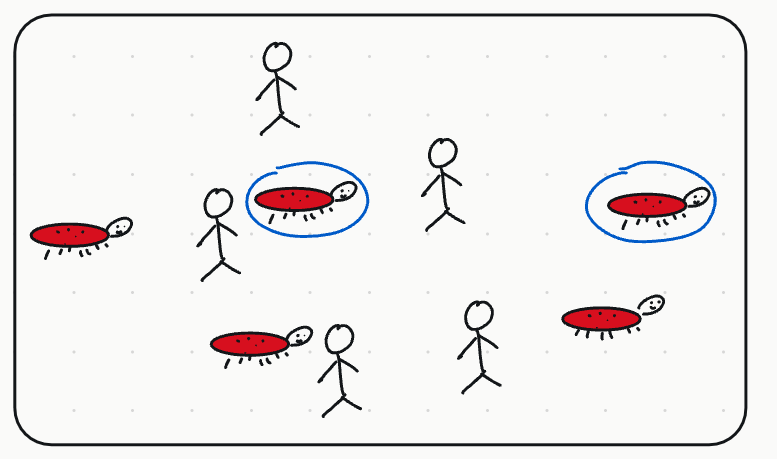
\includegraphics[width=0.4\textwidth]{perfect-precision-2-bugs}
			\end{center}
			Then the precision is
			\begin{align*}
				\text{Precision} := \frac{TP}{PP} = \frac{2}{2} = 1
			\end{align*}
			We achieved 100\% precision, which sounds like we did a great job.
			Meanwhile, there are $5$ humans in total, so the recall is
			\begin{align*}
				\text{Recall} := \frac{TP}{P} = \frac{2}{5} = 0.4
			\end{align*}
			40\% is not a good recall. Note we did not make any false positive
			errors. However we have three false negatives, since we did not
			circle three actual bugs. Thus implicitly we are saying that
			the cost of false positives is higher than the cost of false negatives.
			
			Now say instead that we care more about $FN$. Imagine the model
			circled 8 objects, 5 of which are bugs and 3 of which are humans:
			\begin{center}
				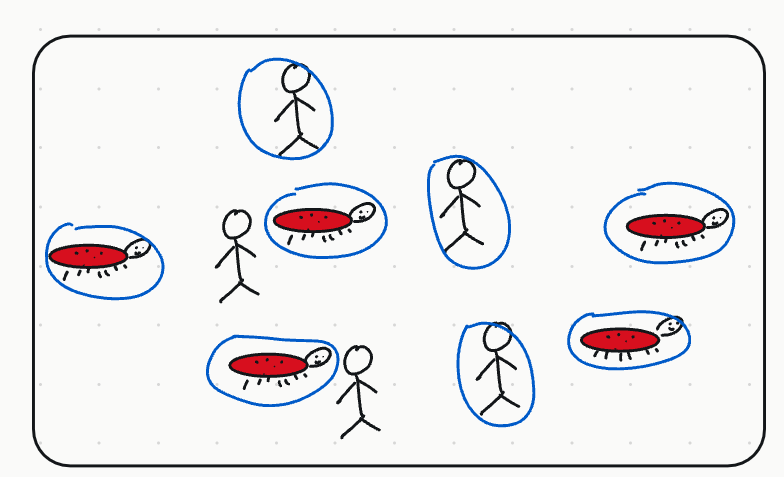
\includegraphics[width=0.4\textwidth]{perfect-recall-5-bugs-3-humans}
			\end{center}
			Then the precision is
			\begin{align*}
				\text{Precision} := \frac{5}{8}
			\end{align*}
			The recall is
			\begin{align*}
				\text{Recall} := \frac{5}{5}
			\end{align*}
			Here we are implicitly saying $FN$ is most costly, because we did
			not make any false negative errors, in spite of making false positive
			errors.
		\end{example}
	\end{tcolorbox}
	We can combine precision and recall into a performance metric $F_1$,
	called the \textbf{geometric average}:
	\begin{align*}
		F_1 := \frac{2}{\frac{1}{\text{Recall}} + \frac{1}{\text{Precision}}}
	\end{align*}
	Another useful metric is \textbf{False Discovery Rate (FDR)}, the proportion
	of mistakes when $\hat{y}=1$:
	\begin{align*}
		FDR := \frac{FP}{PP}
	\end{align*}
	(Note $\text{FDR} = 1 - \text{Precision}$).
	Related to $FDR$ is the \textbf{False Omission Rate (FOR)}, the proportion
	of mistakes when $\hat{y}=0$:
	\begin{align*}
		FOR := \frac{FN}{PN}
	\end{align*}
	$FOR$ and $FDR$ also trade-off effectively, similar to how precision and recall
	trade-off.	 Say we weigh $FP$ more heavily than $FN$ ($C_{FP} > C_{FN}$). In that case,
	we are discouraged from making $FP$ predictions, so we will be less inclined
	to predict $\hat{y}=1$, and more $\hat{y}=0$. Thus, the number of $FP$ decreases
	and the number of $FN$ increase, meaning $FOR$ increases. If instead we
	decide that $C_{FN} > C_{FN}$, then we will do the opposite.
	
	Another performance metric $C$ is called the \textbf{total cost}:
	\begin{align*}
		C := C_{FP} \cdot FP + C_{FN} \cdot FN
	\end{align*}
	The \textbf{average cost} $AC$ is the cost incurred per prediction:
	\begin{align*}
		AC = \frac{C}{n}
	\end{align*}
	We are concerned with how to tailor our algorithm to minimize the total cost,
	which in turn accounts for $FP$ and $FN$ costs.
	
\end{document}